\section
 {\href{https://pavlogradmrada.dp.gov.ua/}%
	{Павлоград}}

\Authors{Муляр Дмитро Сергійович}
\aff{"Гімназія №2 з дошкільним відділенням Павлоградської міської ради", Павлоградська ТГ., Павлоградський р-н., Дніпропетровська обл.}
\Address{}{\href{mailto:v.i.mylyar585@gmail.com}{v.i.mylyar585@gmail.com}}
\begin{center}
	\begin{tabular}{| l | c |}
		\hline
		Засноване  & 1779 р.\\ 
		\hline
		Населення & 105 238 \\ 
		\hline 
		Площа & 59,3 км² \\   
		\hline
	\end{tabular}
\end{center}

\subsection{Історія міста Павлоград}
\textbf{Павлоград} — місто в Дніпропетровській області України, адміністративний центр Павлоградського району, розташоване в межиріччі річок Самара і Вовчаю. Площа міста - 59,3 км². Населення - 105 тис. осіб. Відстань до Києва - 529 км.
\begin{itemize}
	\item \textbf{Козацька доба} Близько 1660 р. Кіш Запорізький на території сучасного Павлограда організував перевіз через річку Вовчу. Саме тут проходив таємний козацький шлях на Кальміус і Кагальник.
	
	Після татарських набігів 1768 та 1769 р. ця місцевість тимчасово спорожніла.
	
	На початку 1770 року запорожець, військовий старшина Матвій Хижняк побудував тут зимівник, від якого пішли Матвіївські хутори, а пізніше після ліквідації Запорозької Січі — слобода Матвіївка Азовської губернії. Хижняк розпланував розташування слободи, виділив місце для церкви з дзвіницею, школою та шпиталем, призначив вулиці та місця для побудови будинків слобожан і запросив сімейний та осілий народ селитися в слободі та влаштовуватись будинками і садибами. Першими поселенцями у цій місцевості були запорожці Самарської та Кальміуської паланок, а також демобілізовані військові, які займалися скотарством і рільництвом.
	\item \textbf{Павлоград у часи Української революції 1917–1921 рр.}
	
	Докладніше:\href{https://uk.wikipedia.org/wiki/%D0%97%D0%B0%D1%85%D0%BE%D0%BF%D0%BB%D0%B5%D0%BD%D0%BD%D1%8F_%D0%B1%D1%96%D0%BB%D1%8C%D1%88%D0%BE%D0%B2%D0%B8%D0%BA%D0%B0%D0%BC%D0%B8_%D0%9F%D0%B0%D0%B2%D0%BB%D0%BE%D0%B3%D1%80%D0%B0%D0%B4%D0%B0}{Захоплення більшовиками Павлограда}
	
	Тобто, павлоградська «Просвіта» мала такі самі повноваження, як і катеринославська. Вона мала свої філії в Лозовій, Петропавлівці, Межовій, Васильківці, а також майже в усіх великих селах Павлоградського повіту. При павлоградській «Просвіті» існував просвітянський хор під керівництвом Пантелієва, театральна трупа під керівництвом М. Хмари. «Просвіта» влаштовувала для павлоградців так звані вечори «балачок-бесід». Такі вечори проводилися в помешканні жіночої гімназії (сучасний Будинок творчості), де збиралося до 300 чоловік. На таких вечорах проводилися лекції, концерти, художні читання. «Просвіта» розповсюджувала українські книжечки серед населення, влаштовувала українознавчі курси для учнів шкіл і бажаючих. До переліку активних просвітян належали: В. Самійленко, Твердохліб, В. Благонадьожин, М. Крайнюков, Бачинський, Л. Кизима, Онищенко, Т. Деніщенко, Б. Луцюк, М. Сопряжинський, Є. Кирейко, М. Хмара, Пантелієв, Селіванський, П. Воронін.
	
	\textbf{20 листопада 1917 р.} Павлоград увійшов до складу Української Народної Республіки.
	
	\textbf{18 грудня 1917 року,} російські комуністи-більшовики та об'єднанний загін, що складається з харківських, путіловських червоногвардійців, петроградських червоногвардійців Московської застави, загону солдатів з 30-го піхотного полку, 3-ї Брянської артилерійської батареї та одного бронепотягу, з боєм захопили владу в місті. Загоном командував кадровий офіцер, капітан П. В. Єгоров
	
	\textbf{17 квітня 1918 року} Кримська група Армії Української Народної Республіки під командуванням підполковника Петра Болбочана (див. мал. \ref{fig:Petro_Bolbochan}) звільнила місто.
	
\begin{figure}[h]
	\centering
	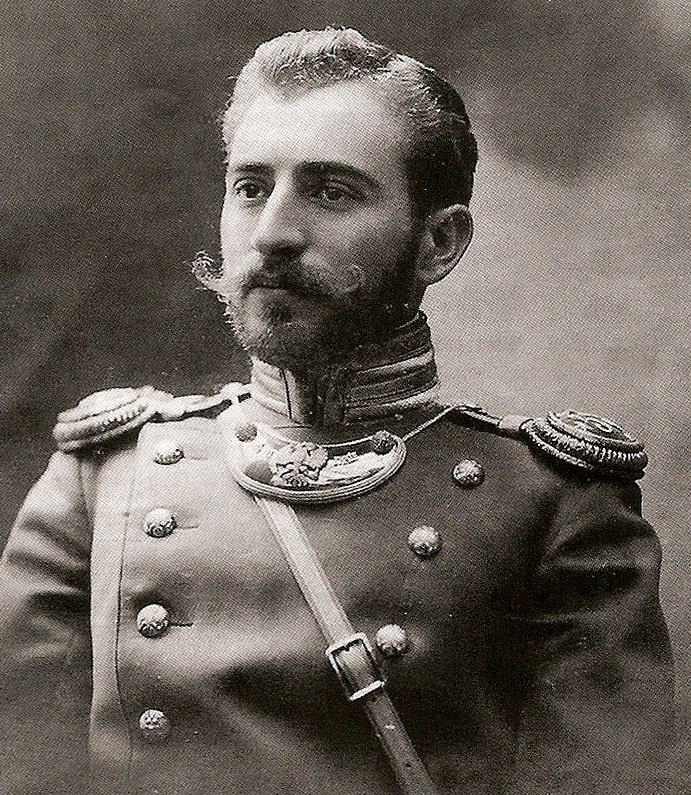
\includegraphics[width=0.6\linewidth]{./images-mylyar/Petro_Bolbochan.jpg}
	\caption{
		\centering
		Підполковник Петро Болбочан, визволитель Павлограда від російсько-більшовицької окупації в 1918 р.}
	\label{fig:Petro_Bolbochan}
\end{figure}

	\textbf{26 грудня 1918 року} у місті стався погром, під час якого було вбито багато євреїв. В результаті за радянських часів багато євреїв залишили місто.
	
	\textbf{У липні 1919 року} Павлоград знову був захоплений білими. На початку січня 1920 року 14-та радянська армія в ході Павлоград-Катеринославської операції відсікла лівофлангову групу Добровольчої армії, остаточно посівши місто.
\end{itemize}
\subsection{Освіта і наука}

\textbf{Система освіти міста складається з:}

\begin{itemize}
\item Західнодонбаського інституту Міжрегіональної академії управління персоналом (МАУП);
\item Павлоградського медичного училища;
\item Західно-Донбаського професійно-технічного ліцею;
\item технікуму Національної гірничої академії України;
\item 25 загальноосвітніх навчально-виховних закладів (в тому числі ЗОШ № 1,\ref{fig:wkola} 2, 3, 4, 5, 6, 7, 8, 9, міський ліцей (колишня середня школа № 10), 11, 12, 13, 14, 15, 16, 17, 18, 19, 20, 21, 22, школа-інтернат № 1, міжшкільний навчально-виробничий комбінат;
\begin{figure}[h]
	\centering
	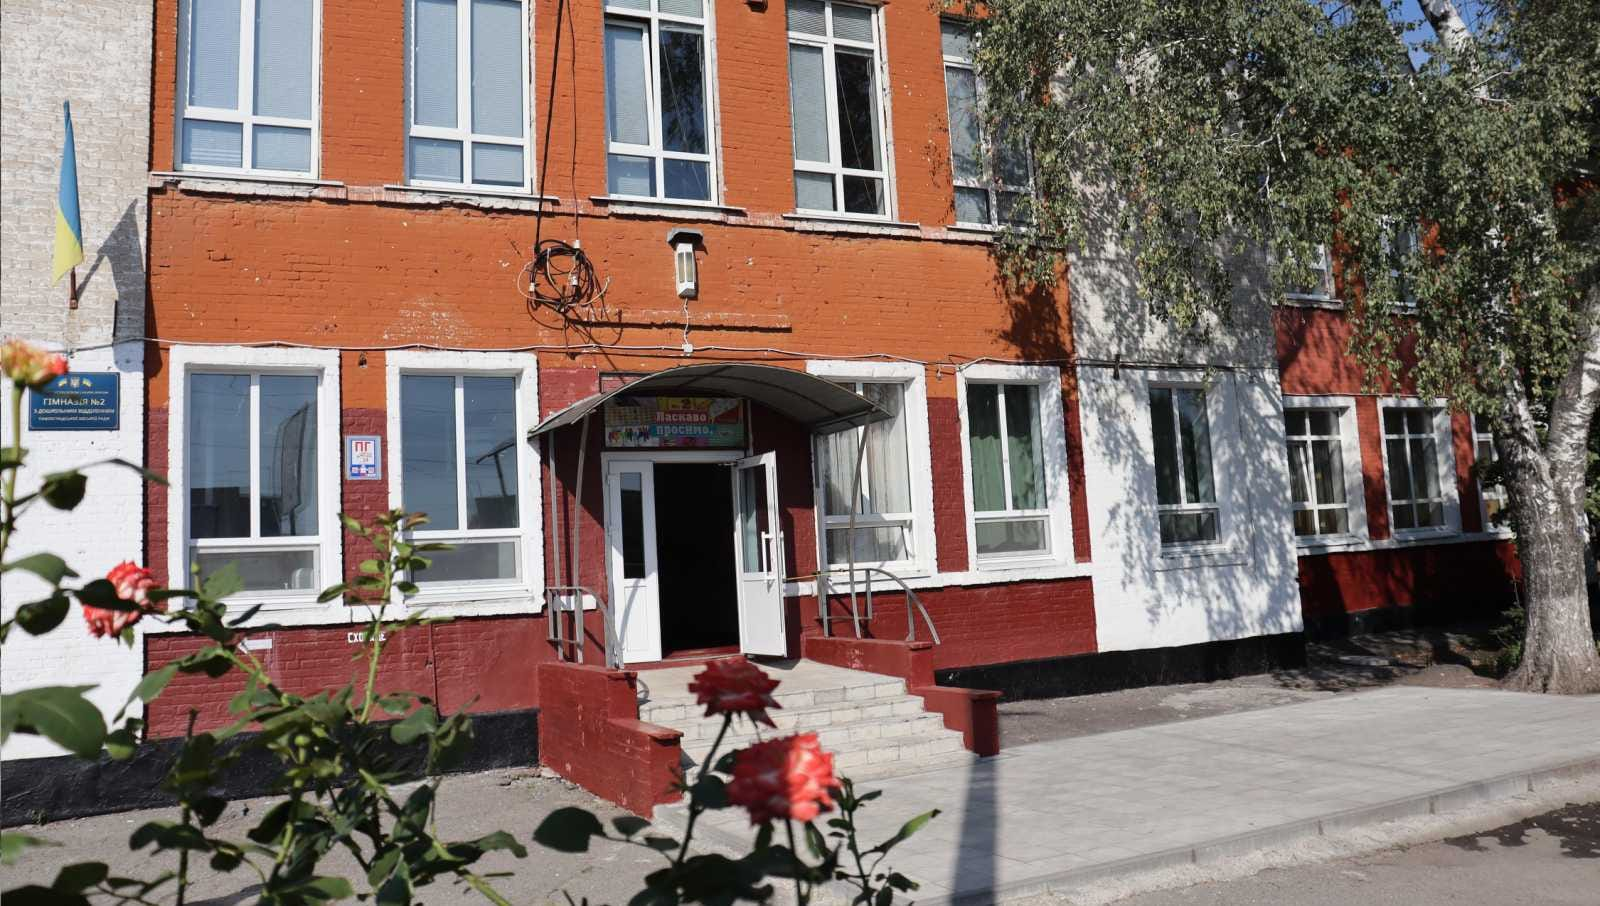
\includegraphics[width=0.6\linewidth]{./images-mylyar/wkola.jpg}
	\caption{
		\centering
		Гімназія №2 з дошкільним відділенням Павлоградської міської ради}
	\label{fig:wkola}
\end{figure}
\item 20 дошкільних установ;
\item позашкільних установ: Палацу творчості дітей та юнацтва, станції юних натуралістів, станції юних техніків.
\end{itemize}
\subsection{Культура}

 Працює Павлоградський драматичний театр ім. Б. Захави, державний історико-краєзнавчий музей, музей поетеси Ганни Світличної (уродженки міста), 2 міські бібліотеки та 7 філій, музична і 2 школи естетичного виховання. У місті знаходяться 27 пам'ятників архітектури — це, переважно, будинки в стилі модерн. Є Храм Нерукотворного Образа (1898 рік), Успенська церква (1986 рік), костьол (90-ті роки XIX ст.). Театр-студія ім. Бориса Захави відсвяткував своє 35-річчя в 2009 році. Режисер театру — заслужений діяч мистецтв України Анатолій Рева.


\textbf{Дитячі і юнацькі колективи, що користуються особливою повагою в місті, країні й за її межами:}
\begin{itemize}
	\item Зразковий ансамбль народного танцю «Юність» (керівник заслужений працівник культури України Кириченко Н. М.);
	\item Народний колектив театру сучасної хореографії «Лик» (керівник Оксень Л. Ю.);
	\item Хореографічний центр «Контрасти» (керівник Оксень Л. Ю.);
	\item Ансамбль бального танцю «Натхнення» (керівник Оксень Л. Ю.);
	\item Зразковий клуб акробатичного рок-н-ролу «Восторг» (керівник Тітова О. В.)
\end{itemize}
	
\textbf{Пріоритетні види спорту: бойовий гопак, бокс, кікбоксинг, важка атлетика, спортивна гімнастика, плавання}
\begin{itemize}
	\item Комунальна бюджетна установа «Міський культурно-дозвільницький центр»
	\item БК Машинобудівників
	\item Комунальний заклад «Павлоградський історико-краєзнавчий музей»
	\item Комунальний заклад "Початковий спеціалізований мистецький навчальний заклад «Дитяча музична школа № 1, 2, 3»;
	\item Комунальний заклад «Павлоградський драматичний театр ім. Бориса Захави»
\end{itemize}
%\begin{figure}
%%%\end{subfigure}
%\end{figure}

\subsection{Джерела та література}
\begin{itemize}
	\item Я. В. Верменич. Павлоград [Архівовано 25 жовтня 2016 у Wayback Machine.] // Енциклопедія історії України : у 10 т. / редкол.: В. А. Смолій (голова) та ін. ; Інститут історії України НАН України. — К. : Наукова думка, 2011. — Т. 8 : Па — Прик. — С. 15. — 520 с. : іл. — ISBN 978-966-00-1142-7.
	\item {\href{https://pavlogradmrada.dp.gov.ua/}%
		{Офіційний сайт Дніпропетровської обласної адміністрації}}
	\item Павлоград — Інформаційно-пізнавальний портал | Дніпропетровська область у складі УРСР [Архівовано 17 березня 2013 у Wayback Machine.] (На основі матеріалів енциклопедичного видання про історію міст та сіл України, том — Історія міст і сіл Української РСР. Дніпропетровська область. — К.: Головна редакція УРЕ АН УРСР, 1969. — 959 с.)
	\item Вулиці Павлограда розповідають… : [наук.-іст. довід.] / Т. Ведмідь, Л. Губарєва. — Павлоград: Арт Синтез-Т, 2017. — 211 с. : іл., табл., портр.
\end{itemize}